\subsection{Erschütterungen}

\begin{frame}
\frametitle{Erschütterungsemissionen/-immissionen}
\begin{center}
 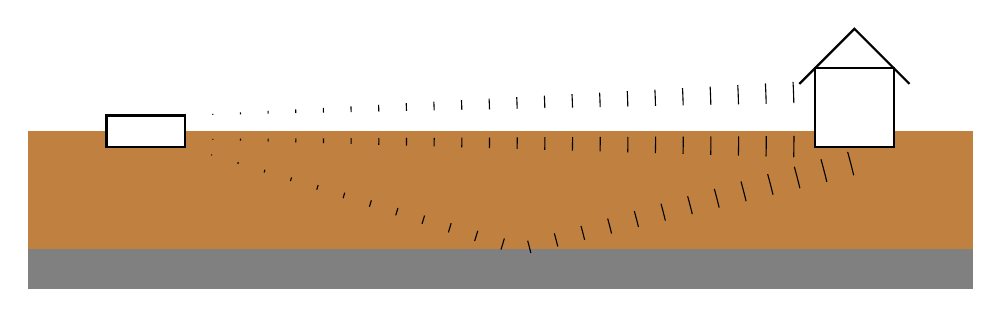
\begin{tikzpicture}
 \fill[color=brown] (-6,-1.5) rectangle (6, 0);
 \fill[color=gray] (-6,-2) rectangle (6,-1.5);
 \draw[thick, fill=white] (-5,-0.2)  rectangle (-4, 0.2);
 \draw[thick, fill=white] ( 4,-0.2)  rectangle ( 5, 0.8);
 \draw[thick] (3.8, 0.6) -- (4.5, 1.3) -- (5.2, 0.6);
 \draw[decorate,decoration={expanding waves, angle=1}] (-4, 0.2) -- (4, 0.5);
 \draw[decorate,decoration={expanding waves, angle=1}] (-4,-0.1) -- (4,-0.2);
 \draw[decorate,decoration={expanding waves, angle=1}] (-4,-0.2) -- (0.25,-1.5) -- (4.5,-0.4);
\end{tikzpicture}

\end{center}
\begin{description}[leftmargin=!,labelwidth=1mm]
\item[Quellen] Verkehr, Bauarbeiten, Maschinen, Naturereignisse
\item[Übertragungsweg] Boden (Dämpfung, Reflexion, Transmission) und Luft (hier nicht betrachtet) 
\item[Empfänger] Gebäude(teile), Lebewesen, Geräte
\end{description}
\end{frame}


\begin{frame}
\frametitle{Erschütterungsemission {\normalsize durch Verkehr}}

\only<1>{
Logarithmische Darstellung der Partikelgeschwindigkeit \cite{studer2008bodendynamik}
\begin{equation*}
 L_v=\mathrm{dB}(v)=20\log\left(\frac{v}{v_\mathrm{ref}}\right)
\end{equation*}
bezogen auf den Referenzwert $v_\mathrm{ref}=\SI{1e-6}{\milli\metre\per\second}$ (ISO 1683).
Damit folgende Übertragungsverluste und -verstärkungen
\begin{equation*}
L_\mathrm{immission}=L_\mathrm{emission}
\underbrace{-\Delta L_{v,\mathrm{geom}}-\Delta L_{v,\mathrm{mat}}- \Delta L_{v,\mathrm{refl}}}_{\text{Verluste im Übertragungsmedium}}
\underbrace{-\Delta L_{v,\mathrm{koppl}}-\Delta L_{v,\mathrm{empf}}}_{\text{Verluste/Verst. am Empfänger}}
\end{equation*}
}

\only<2>{
\includegraphics[width=\textwidth]{fig_img/tunnelspektrum} 
}
\end{frame}


\begin{frame}
\frametitle{Erschütterungsemission {\normalsize durch Bauarbeiten}}
Speziell für Spreng- und Rammerschütterungen \cite{studer2008bodendynamik} ist die Messung an der Quelle schwierig, deswegen wird die eingebrachte Energie als Kenngröße benutzt
\begin{equation*}
 v=cW^\alpha r^\beta.
\end{equation*}
\begin{description}
 \item[$v$] Partikelgeschwindigkeit
 \item[$c$] Koeffizient für Sprengstofftyp (experimentell bestimmt)
 \item[$W$] Sprengstoffgewicht
 \item[$\alpha$] Skalierungsfaktor ($\alpha\approx1/3$)
 \item[$r$] Abstand Quelle -- Empfänger
 \item[$\beta$] Skalierungsfaktor ($\beta=-2$ für Punktquelle)
\end{description}
Maschinen werden nach der gleichen Formel geschätzt \cite{studer2008bodendynamik}.
\end{frame}


\begin{frame}
\frametitle{Erschütterungseinwirkung} %TODO KB Wert
\includegraphics[width=0.88\textwidth]{fig_img/grenzwerte} 
%\cite{studer2008bodendynamik} % Belästigung (subjektiv) vor Schädigung
\end{frame}

\begin{frame}
\frametitle{Erschütterungseinwirkung {\normalsize auf Bauwerke}}
Länderspezifische Richtlinien (Deutschland: DIN 4150-3)

Richt- und Grenzwerte beziehen sich meist auf die Partikelgeschwindigkeit und werden unterteilt nach
\begin{description}
 \item[Häufigkeitsklassen]: gelegentlich, häufig, permanent
 \item[Empfindlichkeitsklassen]: sehr wenig, wenig, normal, erhöht empfindlich  
 \item[Frequenz]: $<\SI{30}{\hertz}$, $\SI{30}{\hertz}$--$\SI{60}{\hertz}$, $>\SI{60}{\hertz}$
\end{description}

\bigskip

Beispiel (nach SN 640312a) für häufige Vorgänge, normale Empfindlichkeit und eine Frequenz von $\SI{45}{\hertz}$ beträgt der Richtwert $v=\SI{8}{\milli\metre\per\second}$.
\end{frame}


\begin{frame}
\frametitle{Erschütterungseinwirkung {\normalsize auf Menschen}}
\includegraphics[width=0.99\textwidth]{fig_img/grenzwerte_schall} 
\end{frame}


%\begin{frame}
%\frametitle{Erschütterungseinwirkung{\normalsize auf Geräte}}
%ISO 8569:1996 Mechanical vibration and shock – Measurement and evaluation of
%shock and vibration effects on sensitive equipment in buildings
%\cite{studer2008bodendynamik}
%\end{frame}


\begin{frame}
\frametitle{Erschütterungsreduktion}
\begin{description}
 \item[Quelle:] optimiertes Sprengschema, Maschinenfundamente, Unterschottermatten, Zusatzmassen
 
 \item[Übertragungsmedium:] \includegraphics[width=0.49\textwidth]{fig_img/schlitz}
 
 \item[Empfänger:] Auflagerung/Fundament, Schwingungstilger 
\end{description}
\end{frame}


\begin{frame}
\frametitle{Beispiel}

\only<1>{
\begin{figure}
\includegraphics[width=0.7\textwidth]{fig_img/beispiel_ramme} 
\caption*{Messpunktanordnung \cite{haupt1986bodendynamik}}
\end{figure}
}%only

\only<2>{
\begin{figure}
\includegraphics[width=0.66\textwidth]{fig_img/beispiel_ruettelwalze} 
\caption*{Geschwindigkeitsignal in drei Raumrichtungen \cite{haupt1986bodendynamik}}
\end{figure}
}%only

\end{frame}


